% From http://tex.stackexchange.com/questions/153933/tikz-mindmap-looks-bad
% Niall McConville - pyCav project
\documentclass[article, 12pt, oneside]{memoir}

\usepackage[a2paper]{geometry}
\usepackage{tikz}
\usetikzlibrary{mindmap}
\pagestyle{empty}
\begin{document}
    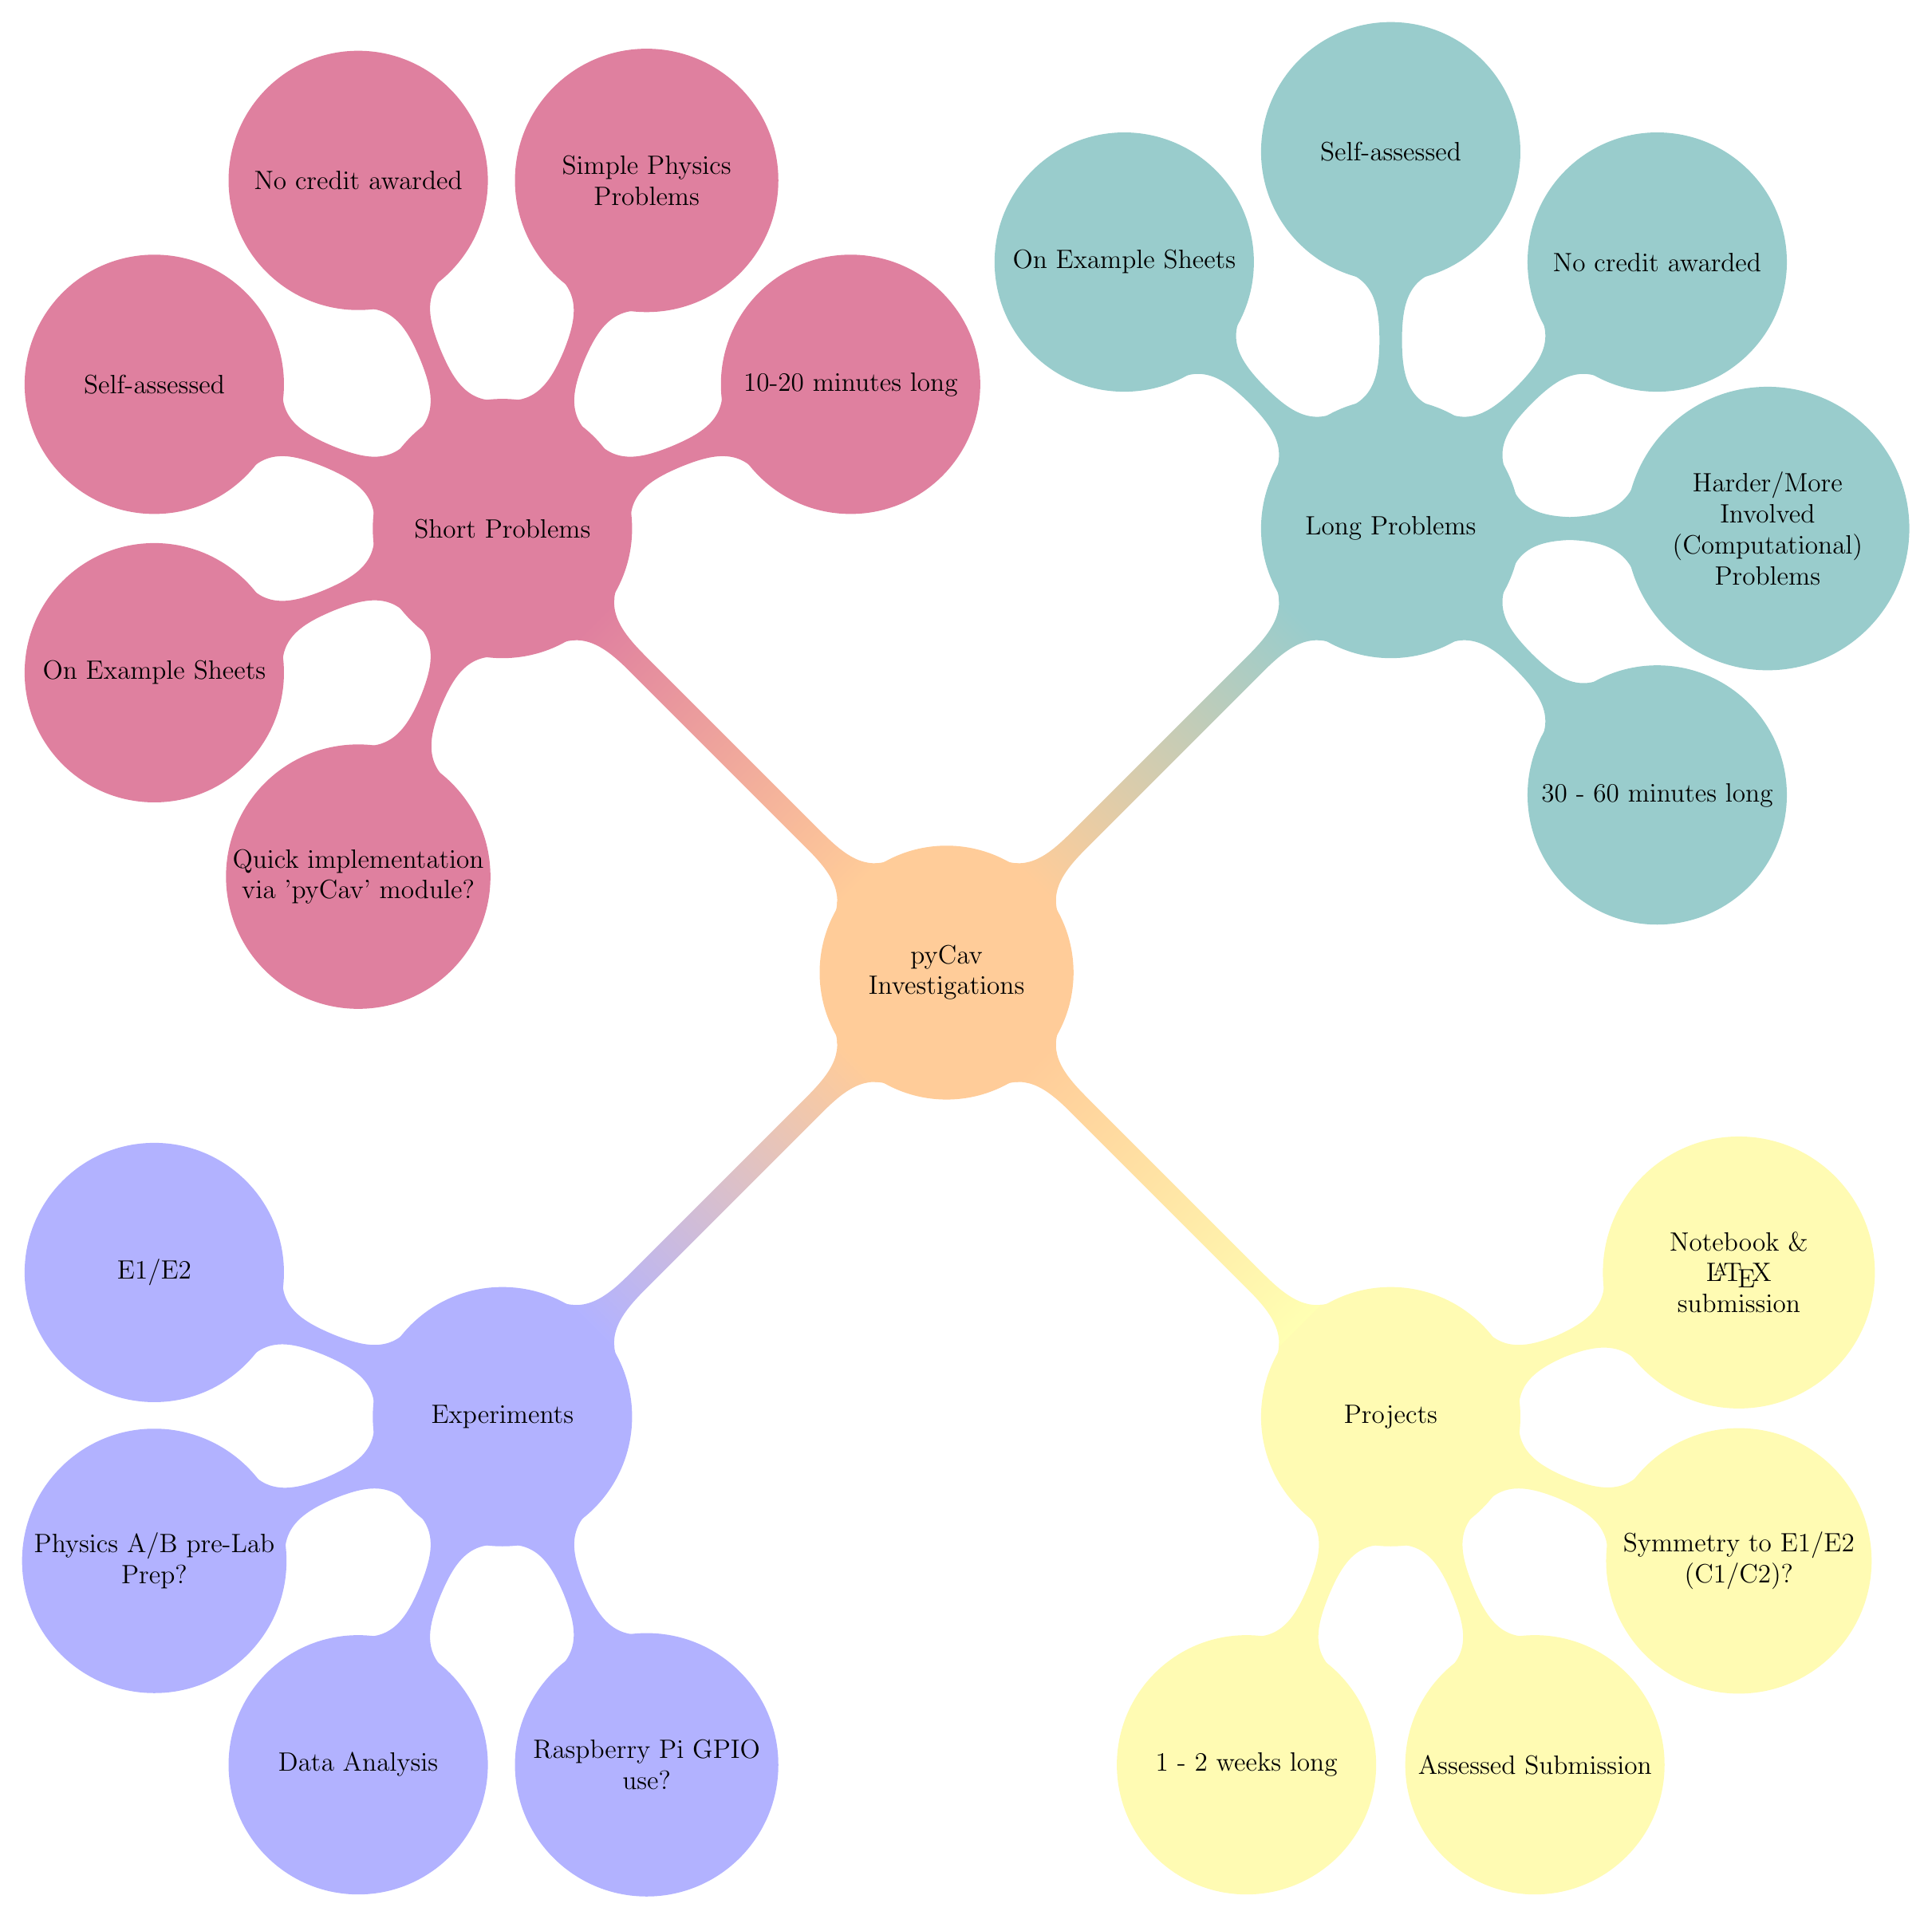
\begin{tikzpicture}[
        mindmap,
        grow cyclic, text width=4cm, align=flush center,
        every node/.style={concept},
        concept color=orange!40,
        level 1/.style={level distance=10cm,sibling angle=90},
        level 2/.style={level distance=6cm,sibling angle=45}]

            \node [root concept] {pyCav\\Investigations}
                child [concept color=blue!30] { node {Experiments}
                    child { node {E1/E2} }
                    child { node {Physics A/B pre-Lab Prep?} }
                    child { node {Data Analysis} }
                    child { node {Raspberry Pi GPIO use?} }
                }
                child [concept color=yellow!30] { node {Projects}
                    child { node {1 - 2 weeks long} }
                    child { node {Assessed Submission}}
                    child { node {Symmetry to E1/E2 (C1/C2)?} }
                    child { node {Notebook \& \\\LaTeX \\submission} }
                }
                child [concept color=teal!40]  { node {Long Problems}
                    child { node {30 - 60 minutes long}}
                    child { node {Harder/More Involved (Computational) \\Problems}}
                    child { node {No credit awarded}}
                    child { node {Self-assessed}}
                    child { node {On Example Sheets}}
                }
                child [concept color=purple!50] { node {Short Problems}
                   child { node {10-20 minutes long}}
                   child { node {Simple Physics Problems}}
                   child { node {No credit awarded}}
                   child { node {Self-assessed}}
                   child { node {On Example Sheets}}
                   child { node {Quick implementation via 'pyCav' module?}
                }
            };
    \end{tikzpicture}
\end{document}